\subsection{DAC Reconstruction Filter} \label{subsec:DAC_Filter}
The stimulus signal used to excite the DUT is generated by an LTC1668 DAC \cite{DAC_LTC1668}. This is a high speed differential current output DAC. To obtain good spectral purity a reconstruction filter is typically fitted on the output of a digital to analog converter.

When an impedance analyzer is testing a DUT, it tests at a specified frequency, this implies that all other frequencies than the test frequency should not be present, i.e. the spectral content of the test signal should be a single spike at the desired frequency. The DAC is capable of more than \SIQ{80}{\decibel} SFDR, Sporious Free Dynamic Range, as seen in figure \ref{fig_7_1_1_SFDR}. This has been deemed more that suitable for the project. 

\begin{figure}[H]
    \centering
    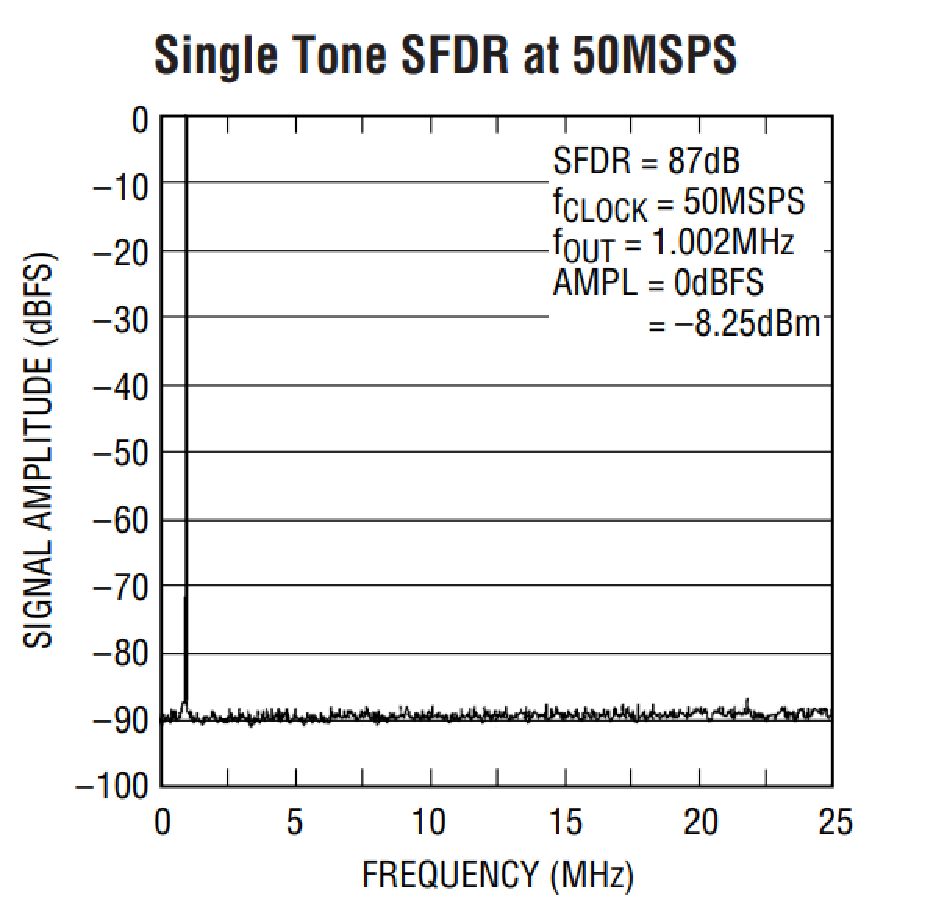
\includegraphics[clip, trim=0 0 0 0, width=0.6\textwidth]{Sections/7_SystemDesign/Figures/7_1_1_DAC_SingleTone_SFDR.pdf}
    \caption{The Sporious Free Dynamic Range, SFDR, of the used DAC given a single tone output frequency.}
    \label{fig_7_1_1_SFDR}
\end{figure}

Such pure frequency generation is however not obtainable without a purposely designed reconstruction filter to remove any high frequency content.

For this porpuse, the DAC is fitted with a 12th order low-pass filter and a common-mode choke to remove any unwanted common mode noise from the high speed data-lines to the DAC. The Filter is designed in two stages, the first stage is a 4th order passive low-pass Butterworth filter, the second is an 8th order low-pass active Chebyshev fitler.

The first part is made of passive components to "loosen" the requirements of the op-amps in the active filters. An op-amps gain rolls of as frequency increases, after the gain bandwidth product, GBW, frequency has been reached the op-amp no longer acts as an amplifier. This can be a bit of a problem, as an active filter no longer necesarrily acts as a filter at frequencies higher than their GBW. A step impulse practically constains the complete frequency spectrum, thus directly sending in sharp edges from the DAC to an active filter can result in some not so predictable hehaviour. Using a passive filter before the active filter removes the sharpest edges, allowing the required bandwidth of the used op-amps to be reduced, op-amps with lower GBW, tends towards a lower cost.

\subsubsection{Passive Recontruction Filter}
The passive filter of the DAC has been designed as a normalized filter that has then been frequency and impedance scaled accordingly. The pass-band of the filter is at \SIQ{1.5}{\mega\hertz}, the stop-band at \SIQ{20}{\mega\hertz} and the attenuation at the stop-band is \SIQ{80}{\decibel}. As previously mentioned the DAC has a differential output. It is desired to keep the entire measurement path differential, and as such the DAC output filter must also be a differential filter. The complete analog DAC filter with common mode choke can be seen on figure \ref{fig_7_1_1_DAC_PASSIVE}. The method used to design the passive filter can be seen in appendix \ref{App:DAC_PASSIVE_FILTER}.

\begin{figure}[H]
    \centering
    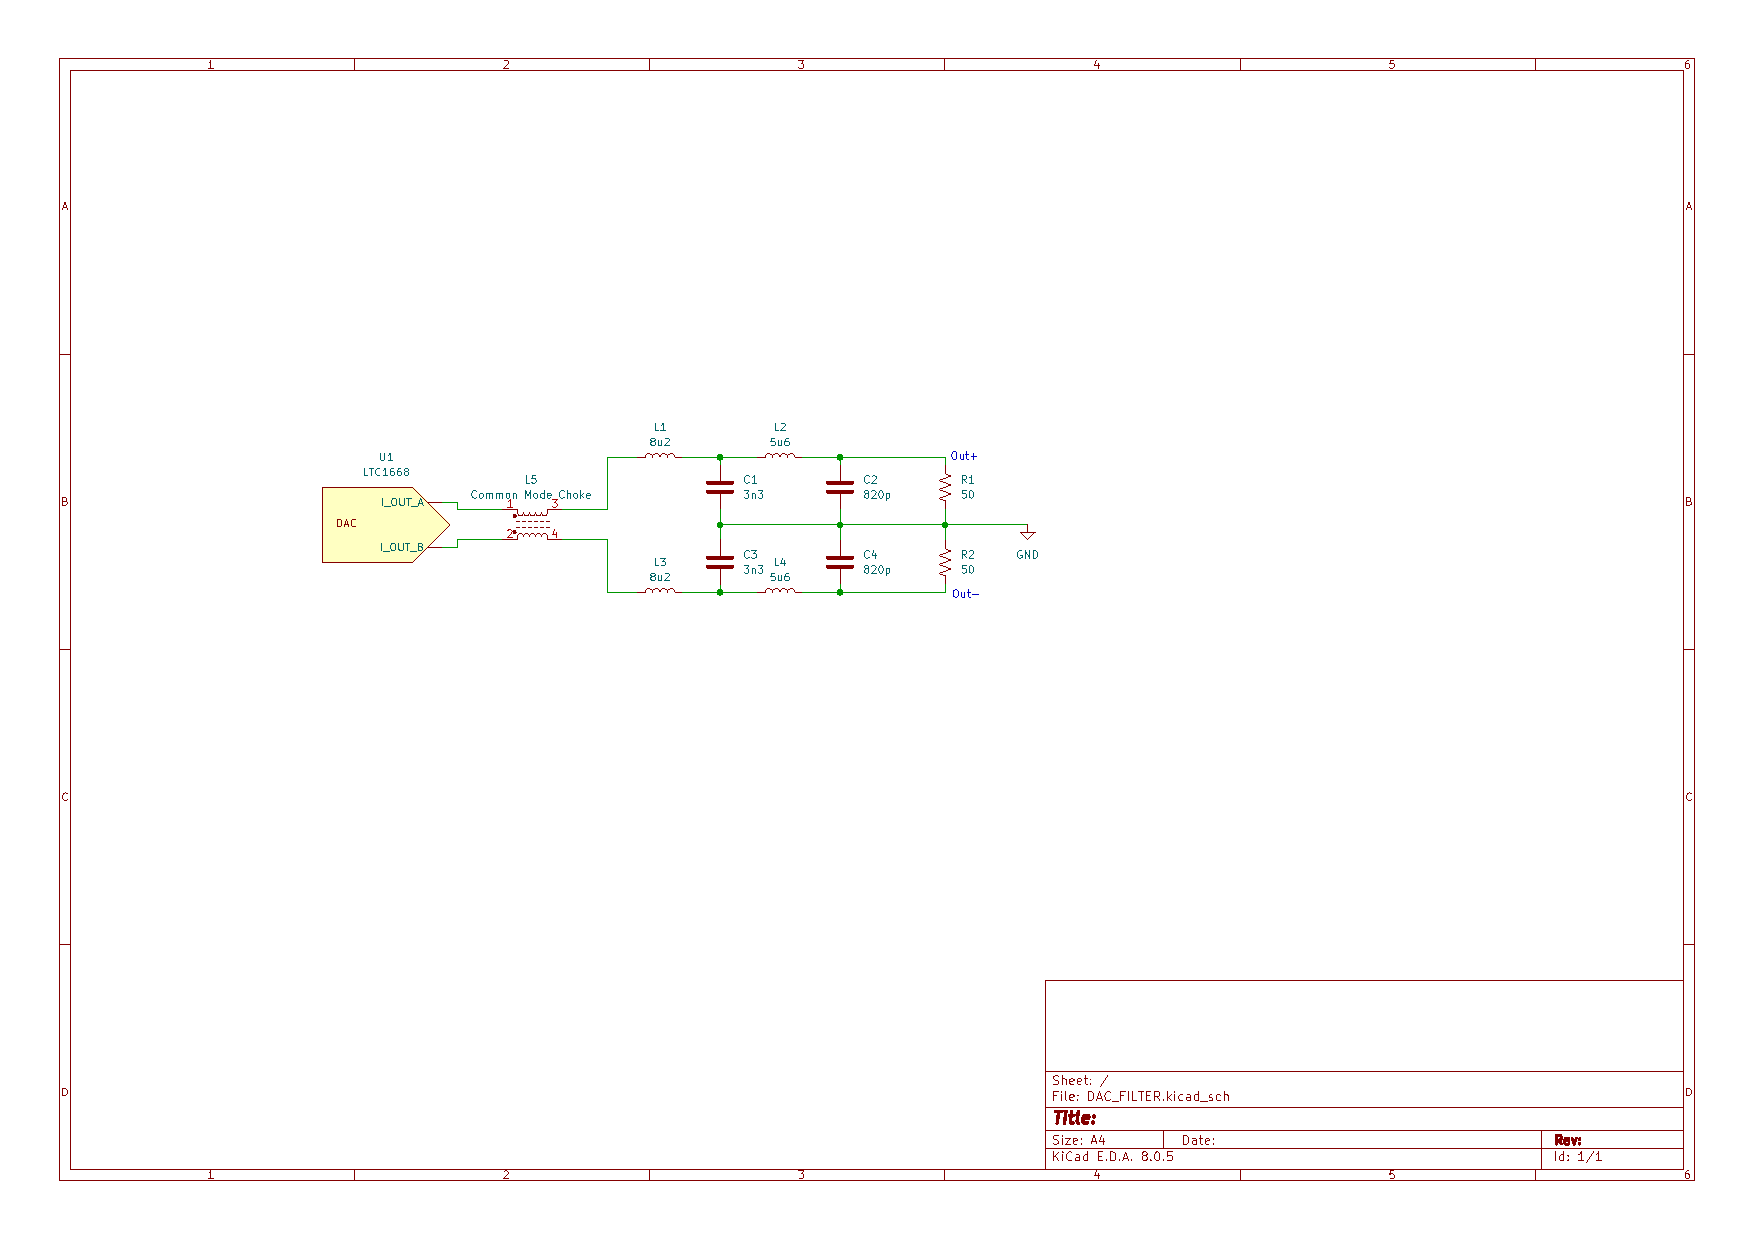
\includegraphics[clip, trim=150 300 250 200, width=0.9\textwidth]{Sections/7_SystemDesign/Figures/7_1_1_DAC_PASSIVE_FILTER.pdf}
    \caption{The 4th order differential passive filter with a common mode choke.}
    \label{fig_7_1_1_DAC_PASSIVE}
\end{figure}

The calculted frequency and step response of the passive filter can be seen in figure \ref{fig_7_1_1_DAC_PASSIVE_RESPONSE}. The step response clearly show how the response to a Heaviside step function is slowed down by the passive filter, i.e. limiting the high frequency components as expected.

\begin{figure}[H]
    \centering
    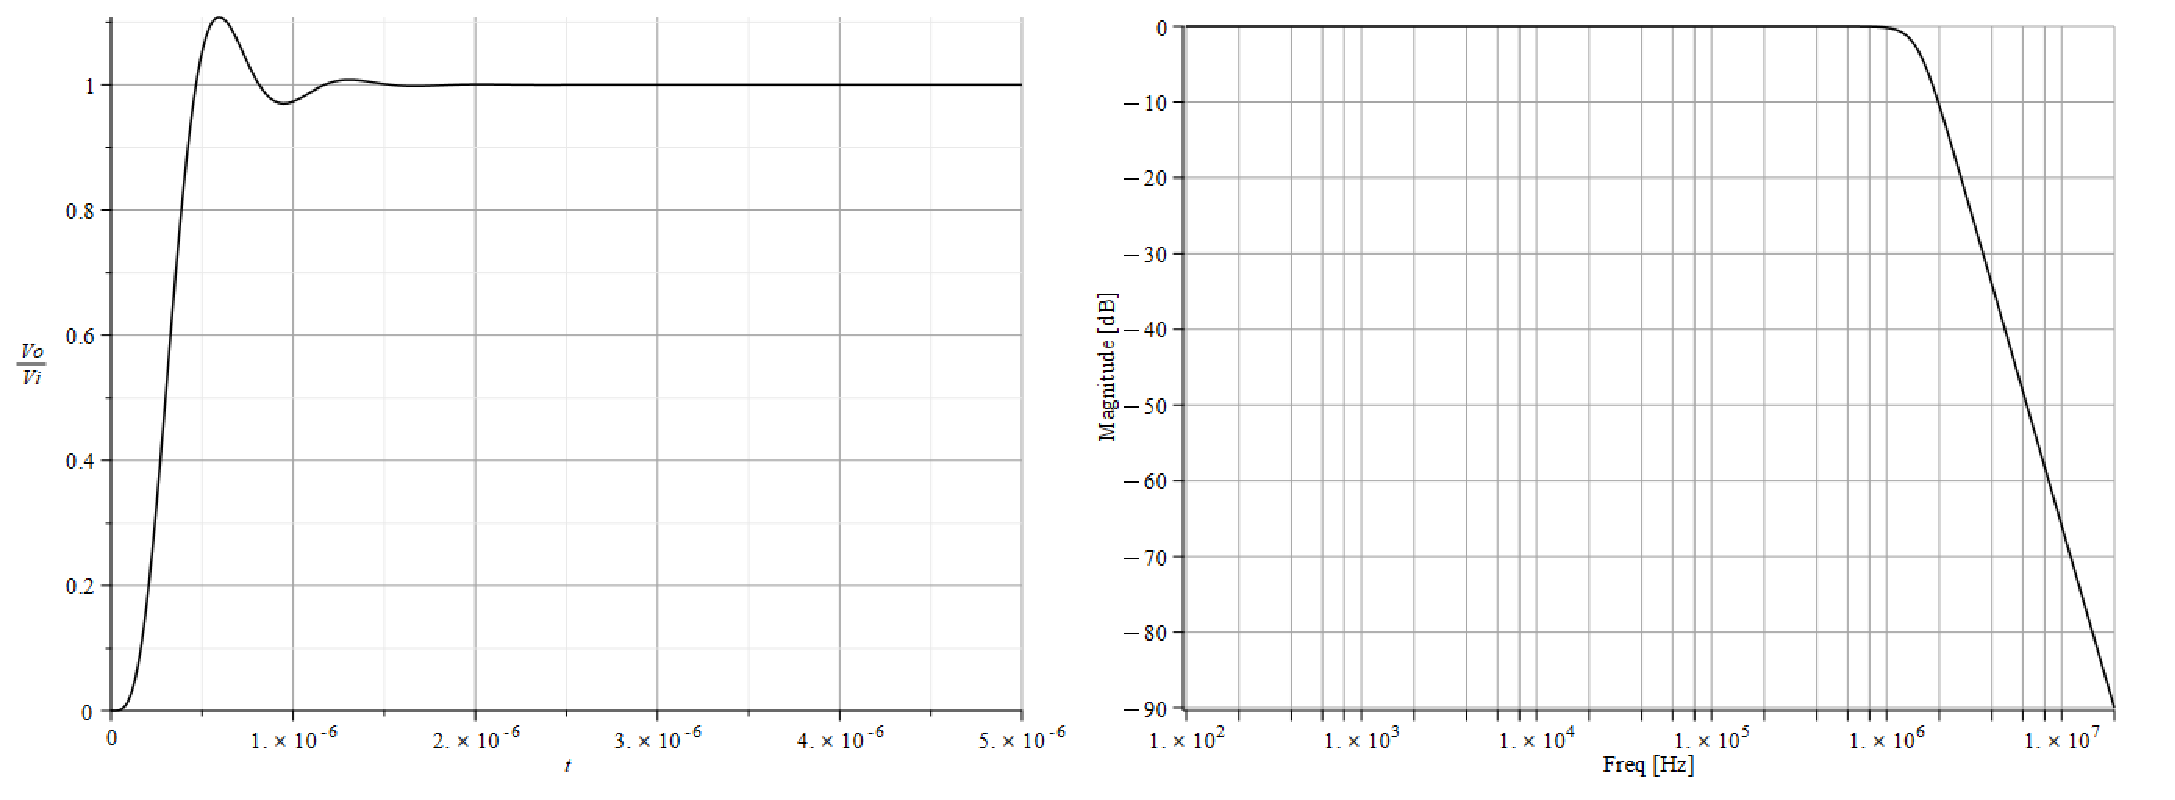
\includegraphics[clip, trim=0 0 0 0, width=1\textwidth]{Sections/7_SystemDesign/Figures/7_1_1_DAC_PASSIVE_RESPONSE.pdf}
    \caption{Step response and frequency response of the passive DAC recontruction filter.}
    \label{fig_7_1_1_DAC_PASSIVE_RESPONSE}
\end{figure}


\subsubsection{Active Reconstruction Filter}
The 8th order active Reconstruction filter handles both filtration and amplification. Both output A and B of the LTC1668 can only swing in the range of \SIQ{0}{\volt} to \SIQ{-1}{\volt}, with a full-scale output current of \SIQ{10}{\milli\ampere}. Thus the full-scale output sinewave will have a DC offset of \SIQ{-500}{\milli\volt}. To remove this, the active filter is AC coupled to the passive filter. The active filter will have a gain of 5 times, such that the output voltage of the DAC and reconstruction filters is \SIQ{5}{\volt pp}.

Quite a few filters have been designed for this project, to accelerate the filter design, Texas Instruments online filter designer has been utilized for the active DAC filter \cite{TI_FILTER_TOOL}. The desgin parameters has been set to 8th order Chebyshev Sallen Key topology, with pass-band at \SIQ{2.5}{\mega\hertz} and a ripple of \SIQ{0.25}{\decibel}. The schematic of the Active filter can be seen in appendix \ref{App:DAC_FILTER}.

The Response of the total DAC reconstruction filter, i.e. both the passive and active filter has been simulated using LTspice from analog devices. The op-amp used is the OPA4830 from Texas Instruments. This op-amps behaviour has been approximated in the simulation as a dual-pole op-amp with \SIQ{100}{\mega\hertz} open-loop GBW, \SIQ{45}{\degree} phase margin and \SIQ{76}{\decibel} open loop DC gain. The differential input to output frequency response can be seen in figure \ref{fig_7_1_1_DAC_SIM_RESPONSE}. The magnitude response is fairly flat up to the maximum output frequency of \SIQ{1}{\mega\hertz} as desired.

\begin{figure}[H]
    \centering
    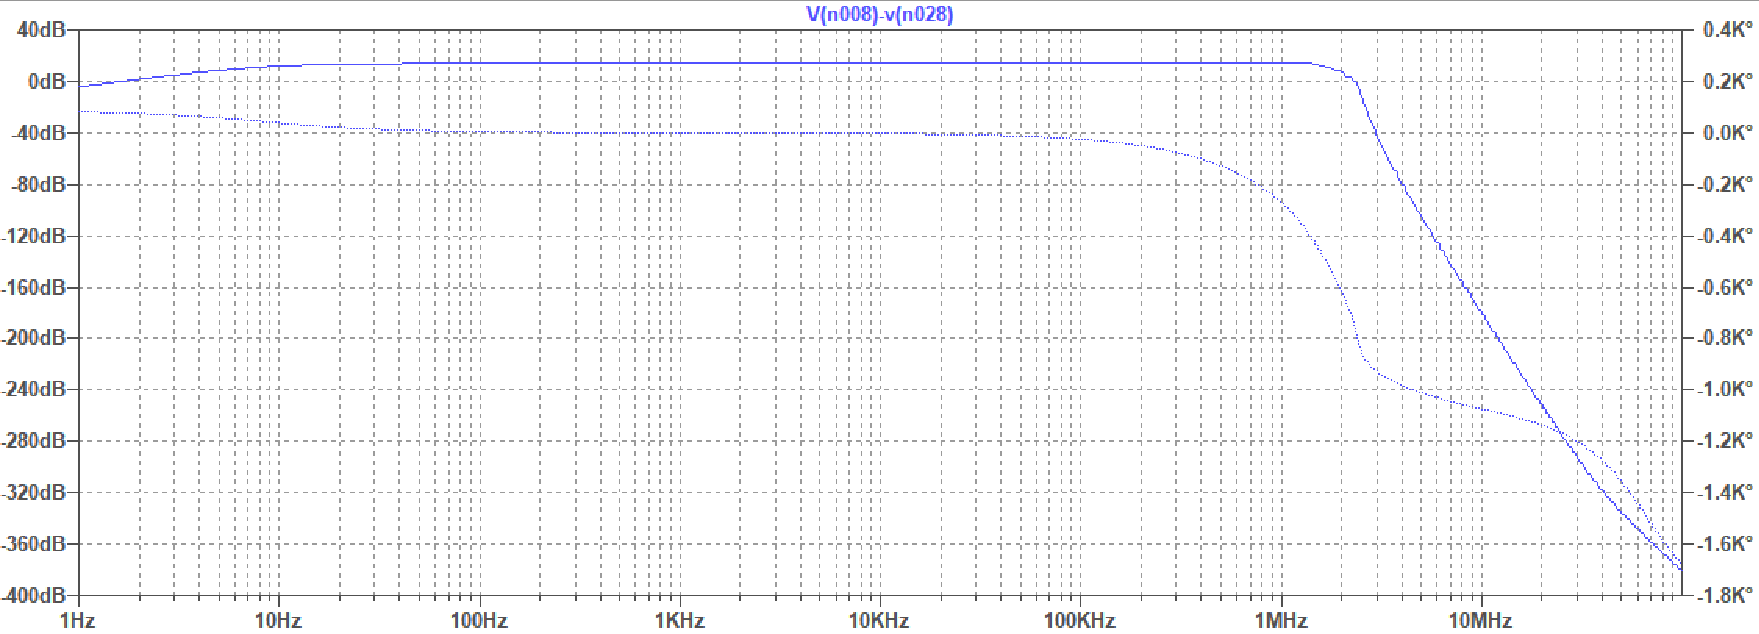
\includegraphics[clip, trim=0 0 0 0, width=1\textwidth]{Sections/7_SystemDesign/Figures/7_1_1_DAC_SIM_FILTER.pdf}
    \caption{Simulated response of the DAC reconstruction filter with op-amp OPA4830.}
    \label{fig_7_1_1_DAC_SIM_RESPONSE}
\end{figure}

One thing to take note of in the simulated frequency response, figure \ref{fig_7_1_1_DAC_SIM_RESPONSE}, is the drastic change in phase at around \SIQ{1}{\mega\hertz}. This indicates a non-constant group delay, giving rise to distortion in the output signal. A transient simulation with a \SIQ{1}{\mega\hertz} signal has been conducted, to analyze the output sinewave of the filter. An FFT analysis has then been performed on this simulated signal, all done with LTspice. The output FFT of the differential signal can be seen in figure \ref{fig_7_1_1_DAC_SIM_FFT}. The FFT indicates no alarming amount of harmonic distortion.

\begin{figure}[H]
    \centering
    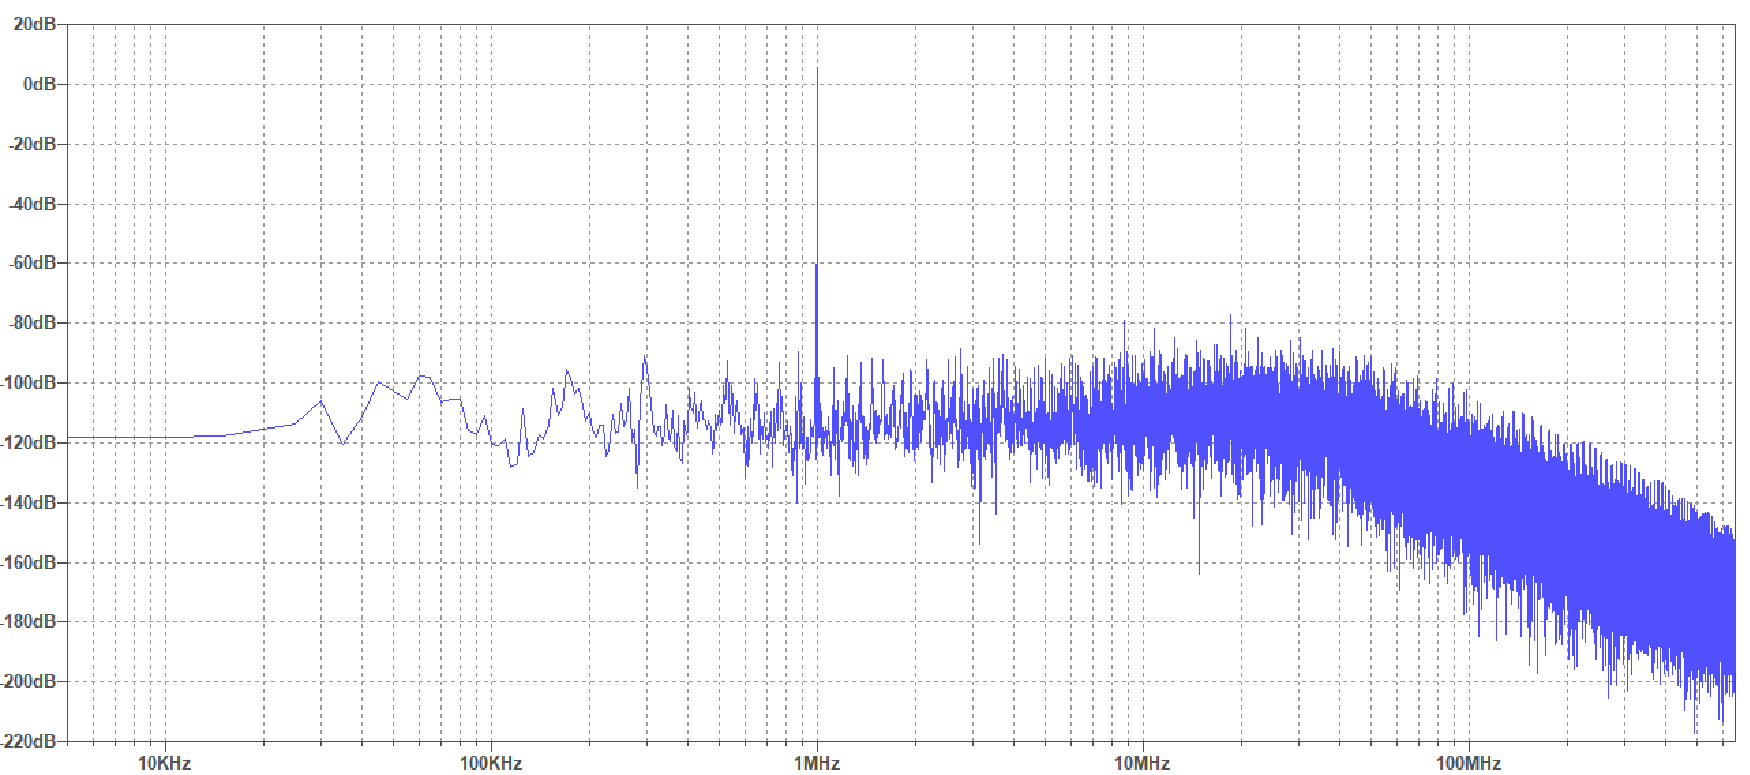
\includegraphics[clip, trim=0 0 0 0, width=1\textwidth]{Sections/7_SystemDesign/Figures/7_1_1_DAC_SIM_FFT.pdf}
    \caption{FFT of the output \SIQ{1}{\mega\hertz} sinewave from a simulated transient response using LTspice.}
    \label{fig_7_1_1_DAC_SIM_FFT}
\end{figure}